\section{Introducción}
\noindent En el capítulo anterior, exploramos las bases tecnológicas y funcionalidades que sustentan el proyecto de evaluación de la viabilidad de JavaCC para el procesamiento de información en la asignatura PIAT. En este nuevo capítulo, nos embarcaremos en un viaje más profundo, adentrándonos en los detalles de la implementación del proyecto, los procedimientos meticulosamente seguidos y el entorno cuidadosamente seleccionado para los desarrollos y las pruebas.

A lo largo de las siguientes secciones, desentrañaremos el proceso de implementación, desglosando los pasos específicos emprendidos durante el desarrollo y revelando el entorno de trabajo cuidadosamente diseñado para garantizar una integración y ejecución exitosas del proyecto. Este recorrido nos permitirá comprender cómo se ha dado vida a esta iniciativa, proporcionando una visión completa de los esfuerzos realizados para alcanzar sus objetivos.

Preparémonos para sumergirnos en el corazón del proyecto, explorando las decisiones tomadas, las herramientas utilizadas y los desafíos superados en el camino hacia la implementación exitosa de JavaCC en PIAT.

\section{Implementación}
\noindent La implementación del proyecto se ha llevado a cabo utilizando el lenguaje de programación Java, aprovechando las capacidades y herramientas que nos proporciona para lograr un desarrollo eficiente y robusto. En esta sección, se profundizará en los detalles de la implementación, destacando las tecnologías clave utilizadas y las decisiones de diseño tomadas para alcanzar los objetivos del proyecto. 

Las tecnologías clave son JavaCC, que nos va a permitir crear analizadores para lenguajes formales; Java, que nos ofrece características como la portabilidad, orientación a objetos y gestión automática de memoria; y un Entorno de desarrollo Integrado (IDE), que nos va a proporcionar las herramientas para desarrollar las prácticas, como el editor de código, compilador, depurador. Hablaremos del entorno utilizado más adelante.

\section{Procedimientos}

\noindent El proceso de implementación se ha dividido en las siguientes fases:

\phantom{text}

\noindent \textbf{Fase 1: Aprendizaje de los conceptos básicos de JavaCC.}

\phantom{text}

\noindent La primera fase consiste en adquirir los conocimientos básicos sobre el funcionamiento de JavaCC, sus conceptos ---qué es un token, un estado léxico, un no-terminal...--- y su sintaxis, incluyendo la definición de gramáticas, la creación de los analizadores léxicos y sintácticos y la generación del código Java. Está fase es considerablemente amplia, ya que hay que dedicarle el tiempo necesario a aprender e interiorizar todos los conceptos y el funcionamiento con esta herramienta.

\phantom{text}

\noindent \textbf{Fase 2: Práctica con JavaCC para crear analizadores léxicos y sintácticos para gramáticas simples.}

\phantom{text}
    
\noindent En la siguiente fase, se realizan ejercicios prácticos para familiarizarse con la herramienta JavaCC y desarrollar la habilidad de crear analizadores léxicos y sintácticos para gramáticas simples. Uno de los ejemplos fue el presentado en la sección \textbf{CALCULADORA}. Realizar estos ejercicios es esencial antes de intentar realizar prácticas más elaboradas, ya que permiten poner en práctica las funcionalidades aprendidas de una manera mas simple y práctica.

\phantom{text}

\noindent \textbf{Fase 3: Aplicación de JavaCC en prácticas de PIAT.}

\phantom{text}

\noindent Una vez se tiene un grado notable de experiencia utilizando la herramienta, en esta fase se aplica JavaCC para desarrollar los analizadores léxicos y sintácticos necesarios para resolver las prácticas de la asignatura PIAT. Esta fase es la más importante y la que más tiempo requiere, ya que se realiza una reingeniería de la práctica ... 


\phantom{text}

\noindent \textbf{Fase 4: Generación de documentación.}

\phantom{text}

\noindent Por último, en la fase 4 se refleja todo el trabajo realizado en las fases anteriores, desde la generación de las gramáticas y su aplicación hasta la validación de resultados y las conclusiones extraídas en cada ejercicio.


\section{Entorno}
\noindent Los desarrollos y las pruebas se han realizado en un entorno de desarrollo integrado (IDE) de Java. En concreto, se ha empleado Eclipse IDE ya que, además de ser el IDE principal con el que se realizan las prácticas de PIAT ---y en general, cualquier práctica relacionada con la programación dentro de la escuela---, existe un plugin de JavaCC que realiza la compilación de los archivos y facilita enormemente el desarrollo. Dicho esto, el lector puede optar por elegir otros editores como Visual Studio Code o Jetbrains, incluso editores de texto como Notepad++, Vim o  nano. Este aspecto queda a gusto del desarrollador. Para la depuración de los analizadores se ha utilizado el debugger del IDE.

Además, para poder realizar los desarrollos necesarios se necesita descargar e instalar la herramienta JavaCC en el equipo. Para saber mas acerca de la instalación y configuración de Elipse IDE con JavaCC, puede consultar el anexo \hyperref[sec:instalaciondejavacc]{\textit{Instalación de JavaCC}}.

En cuanto al equipo de pruebas, se ha elegido un procesador Intel de 8ª generación, el cual cuenta con 6 núcleos y 12 hilos ---este dato es importante a la hora de realizar la validación de resultados en las diferentes prácticas-- con una memoria RAM de 16GB. Estos datos se proporcionan de tal forma que el lector tenga conocimiento del rendimiento de los distintos analizadores en función de  las especificaciones del equipo utilizadas.

\section{Objetivos de la implementación}
\noindent Entre los objetivos principales de la implementación se encuentran el implementar los analizadores léxico y sintáctico para las gramáticas de las prácticas de PIAT, el evaluar la viabilidad de utilizar JavaCC para abordar las prácticas de PIAT, y generar documentación que sirva como recurso para estudiantes y profesores interesados en utilizar JavaCC en proyectos relacionados con el procesamiento de información.

**Una vez claros el entorno utilizado, las especificaciones y configuraciones implementadas en el proyecto, y vistos los objetivos a conseguir en las prácticas, se procederá a analizar el primer caso práctico en el que se puede aplicar JavaCC.

\section{Análisis de ficheros de \textit{log}. Práctica 2}

\noindent El mundo digital genera una gran cantidad de datos, y los logs de sistemas son una fuente importante de información para comprender el comportamiento y el rendimiento de estos sistemas. La práctica 2 de PIAT nos invita a explorar este mundo de datos mediante el análisis de logs de un sistema de correo electrónico. El objetivo de esta práctica es el de aplicar los conocimientos adquiridos sobre expresiones regulares y hacer uso de la programación Java para analizar y extraer información de logs de dicho sistema.

Concretamente, el objetivo de la practica es utilizar expresiones regulares para extraer información estadística y generar informes a partir de los archivos de log del sistema de correo electrónico. La arquitectura del sistema y el formato de los logs se detallan en los anexos \hyperref[sec:P2SistemaCorreo]{\textit{Descripción general del sistema de correo electrónico}} y \hyperref[sec:logscorreo]{\textit{Formato de logs. Sistema de correo electrónico}}.


\subsection{Expresiones Regulares. RegEx}

\noindent Las expresiones regulares, también conocidas como Regex, son un lenguaje formal para describir patrones en cadenas de texto. Son como lupas que nos permiten enfocarnos en detalles específicos dentro de un gran volumen de texto, permitiéndonos extraer información relevante de manera eficiente y precisa.

En esta práctica, las expresiones regulares serán nuestras aliadas para navegar por el laberinto de los logs, desentrañando los mensajes y eventos registrados por el sistema de correo electrónico. Definiremos expresiones regulares para identificar diferentes tipos de registros, como mensajes entrantes, mensajes salientes, mensajes infectados, códigos de error y mucho más.

En este contexto, aplicaremos las expresiones regulares para definir los distintos tokens que queremos reconocer y asi conformar la gramática que analizará JavaCC.

\subsection{Descripción de la práctica}

\noindent La práctica se divide en tres partes principales: La obtención de estadísticos generales, cuya función es contabilizar el número de servidores procesados, los  archivos procesados registros procesados y registros con errores de formato; El análisis por tipo de servidor y día, en el que para cada tipo de servidor, se debe calcular y mostrar los siguientes estadísticos por día:

\begin{itemize}
    \item msgIn: Número de mensajes entrantes.
    \item msgOut: Número de mensajes salientes.
    \item msgINFECTED: Número de mensajes infectados con virus.
    \item msgSPAM: Número de mensajes SPAM no bloqueados.
    \item code 4.3.2: Número de intentos de entrega con código de estado 4.3.2 (sobrecarga).
    \item code 5.1.1: Número de intentos de entrega de mensajes  entrantes con código de estado 5.1.1 (dirección de correo electrónico de destino incorrecta).
\end{itemize}

; Y por ultimo, identificar aquellas cuentas de correo internas desde las que se han enviado más de 500 mensajes. Para cada cuenta, se debe mostrar el nombre de usuario y el número de mensajes enviados.

Un ejemplo del resultado a obtener sería el siguiente:

\lstset{inputencoding=utf8/latin1}
\lstinputlisting{code/P2salida.txt}

\subsection{Desarrollo de la práctica}

Una vez comprendido para que se utilizan las expresiones regulares y conocido el contexto de la práctica con el objetivo final, en esta sección se describe cómo se resuelve esta práctica utilizando JavaCC, apoyándonos en el archivo Parser.jj proporcionado.

El primer paso para resolver la práctica es definir la estructura de árbol que seguirá el analizador sintáctico. Esta estructura determina el tipo de traza que se está analizando y las acciones correspondientes a realizar en cada caso. La siguiente figura ilustra esta estructura:

\begin{figure}[H]
    \centering
    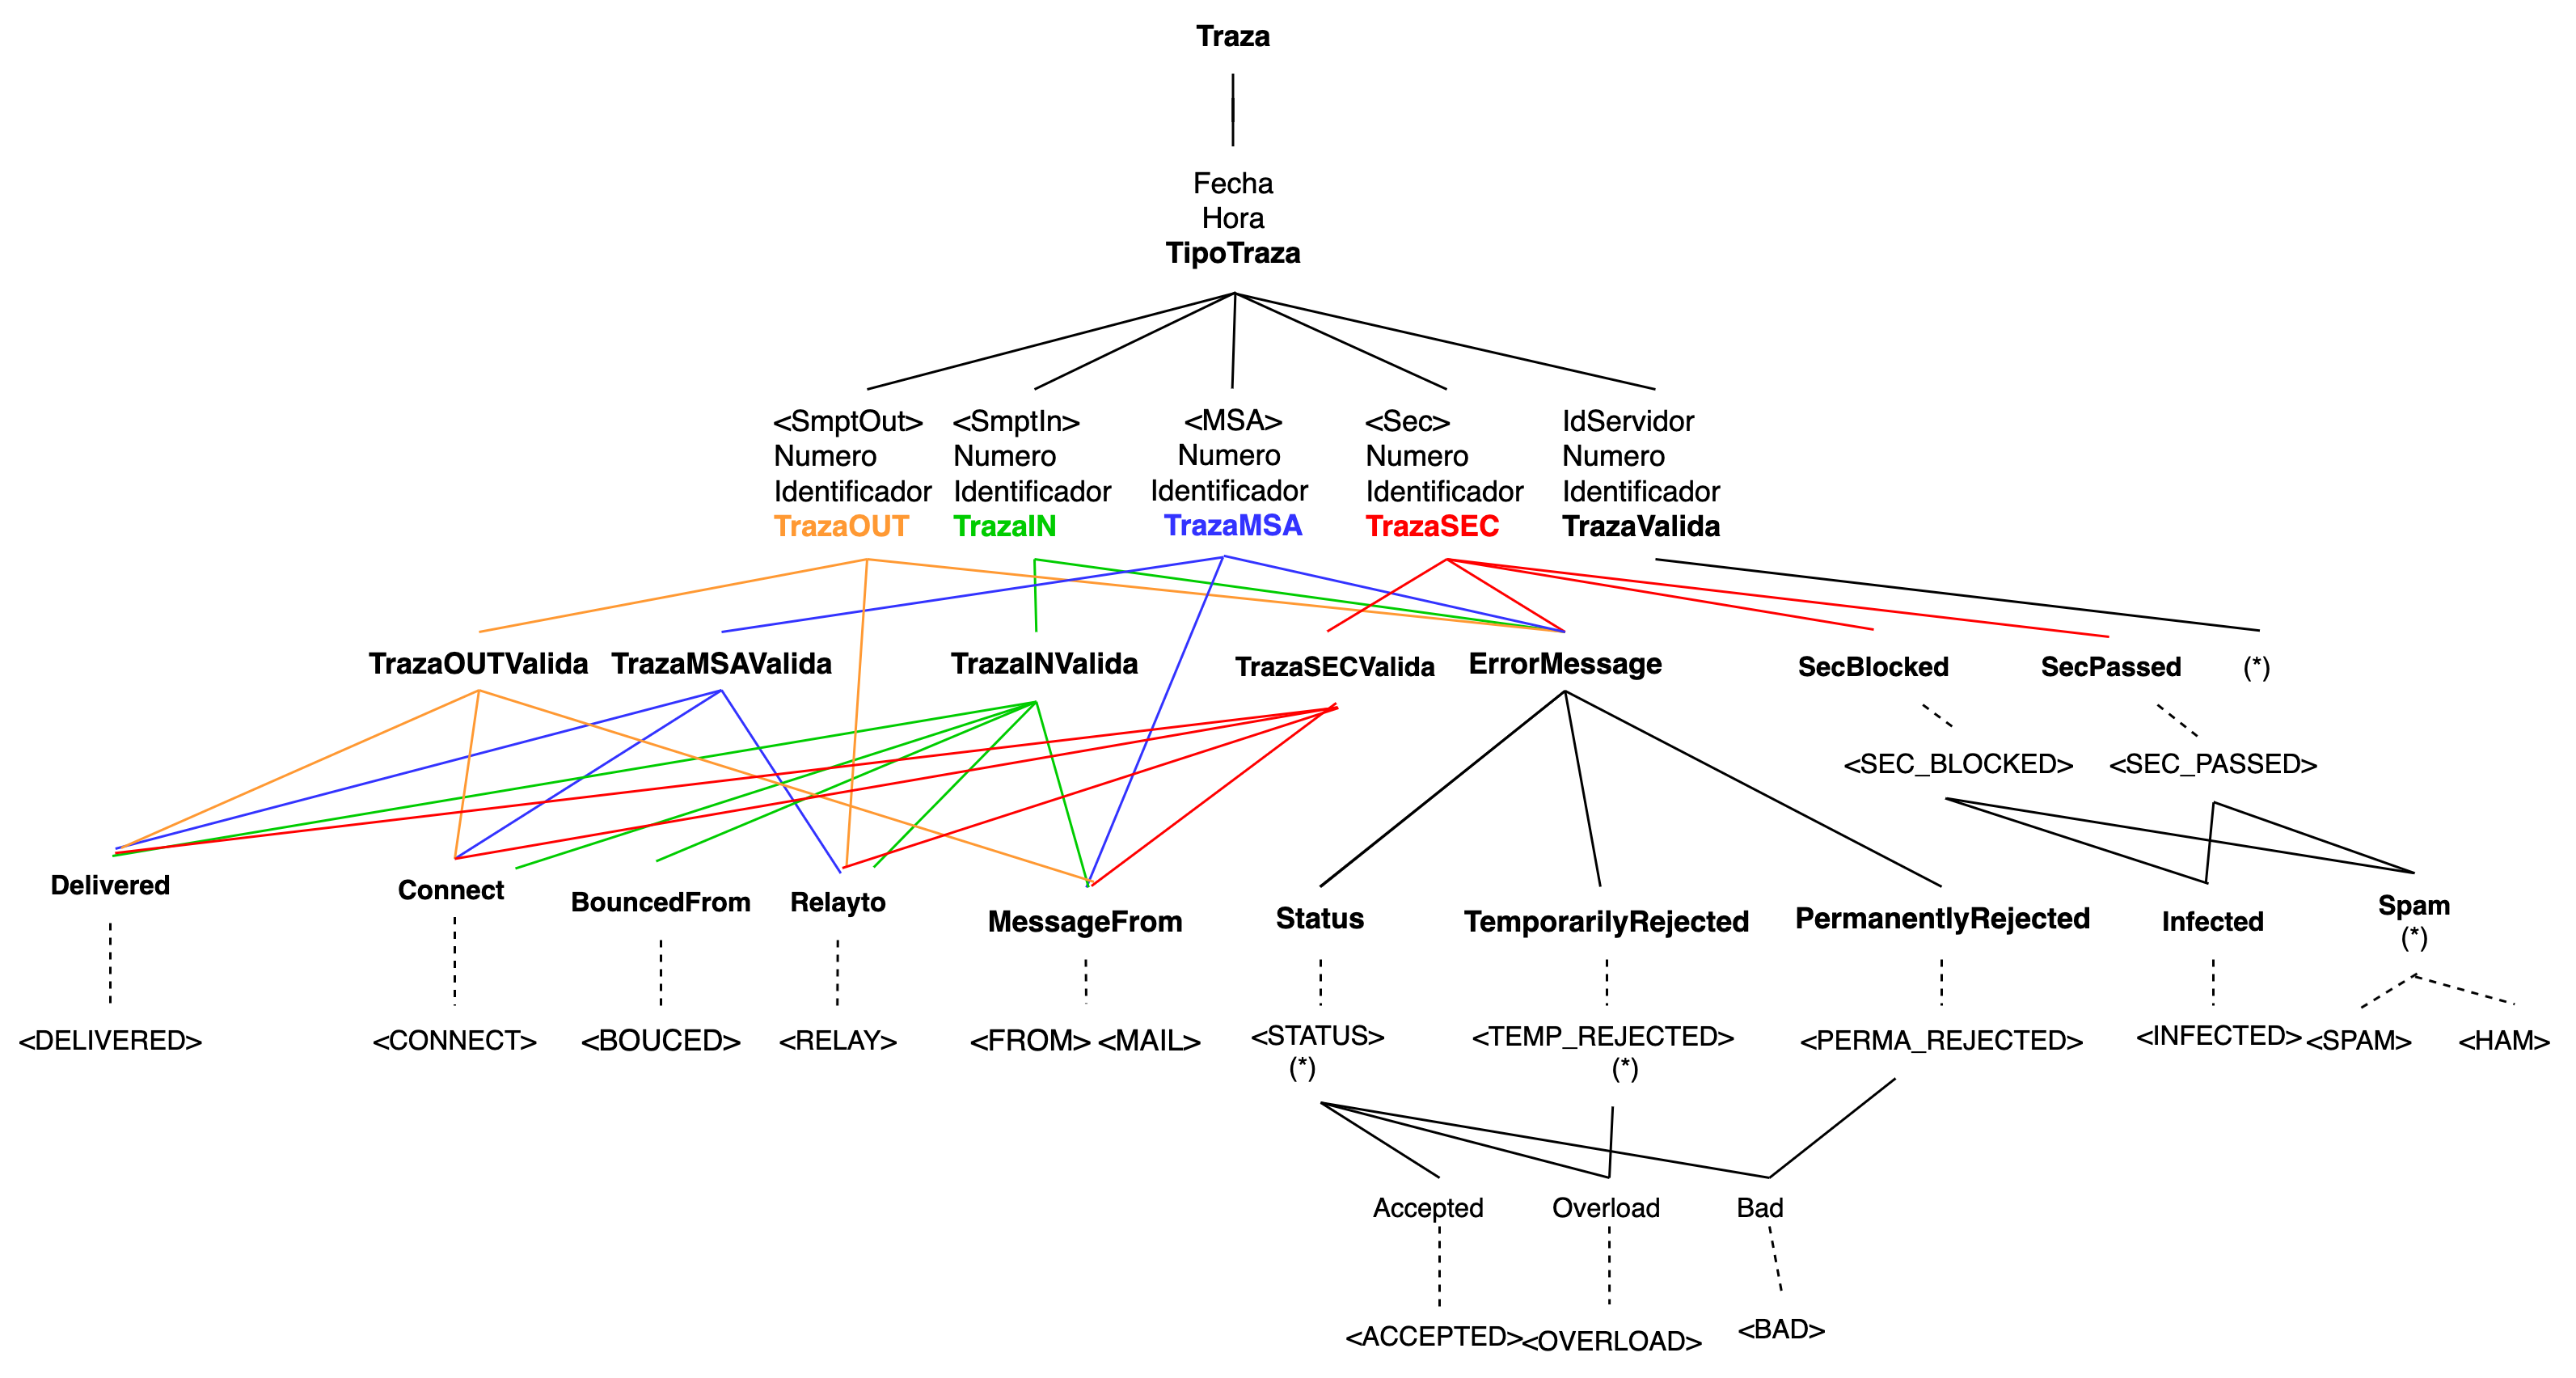
\includegraphics[width=\textwidth]{imagenes/arboltraza.png}
    \caption{Estructura de árbol. Análisis de trazas log.}
    \label{fig:arboltraza}
\end{figure}

Esta figura refleja la estructura del análisis sintáctico, en la que se observa toda la estructura definida a la hora de reconocer las trazas. Se observa como se contemplan cinco tipos de trazas, las \lstinline|msa|, \lstinline|smpt-in|, \lstinline|smpt-out|, \lstinline|security| y otros tipos de servidores. Para cada tipo de traza se definen las distintas posibilidades que puede haber dentro de cada tipo de traza, de tal forma que se describe la estructura de forma detallada. En aquellas ``ramas'' en las que queramos ejecutar alguna acción, como puede ser añadir los valores a un estadístico, se define una acción léxica dentro del no-terminal, como por ejemplo:

\lstset{inputencoding=utf8/latin1}
\lstinputlisting{code/overload.jj}

El archivo Parser.jj define el analizador léxico y sintáctico para procesar los logs. A continuación, se detalla la estructura y las funciones más relevantes del archivo.

En las opciones del analizador se definen configuraciones importantes como la concurrencia, ya que la gramática generada en JavaCC debe tener la capacidad de ejecutarse de forma concurrente para distintas entradas ---en este caso, varios ficheros de log---.

\lstset{inputencoding=utf8/latin1}
\lstinputlisting{code/p2static.jj}

además de incluir varias declaraciones y métodos auxiliares que facilitan el registro y manejo de estadísticas:

\lstset{inputencoding=utf8/latin1}
\lstinputlisting{code/p2declarations.jj}

Los tokens y estados léxicos se definen para identificar y manejar las distintas partes del log. Aquí se muestra un extracto de estas definiciones:

\lstset{inputencoding=utf8/latin1}
\lstinputlisting{code/p2tokens.jj}

Cabe destacar que se utilizan estados léxicos como \lstinline|SERVER|, \lstinline|LEX_MSA|, \lstinline|LEX_IN|, \lstinline|LEX_OUT|... que permiten analizar unicamente ciertos tokens cuando el analizador se encuentra en dicho estado, lo que acelera de forma desmesurada la rapidez del analizador ---lo veremos en la sección de validación de resultados---.

% \textbf{...diagrama o tabla que resuma los estados léxicos y su función...
% }
%  Esto facilitaría la comprensión de la estructura del analizador

% El analizador léxico utiliza diferentes estados para reconocer los tokens de entrada de manera eficiente y precisa.
El estado inicial es DEFAULT, donde se reconocen tokens comunes como espacios en blanco, saltos de línea y fechas.

Al encontrar un token que indica el inicio de un tipo específico de servidor, el analizador cambia a un estado léxico específico para ese servidor. Por ejemplo, al encontrar el token "msa", el analizador cambia al estado LEX\_MSA. Dentro de cada estado de servidor (LEX\_MSA, LEX\_IN, LEX\_OUT, LEX\_SEC), se reconocen tokens específicos relacionados con ese tipo de servidor, como ``message from:'' en LEX\_MSA o ``bounced from:'' en LEX\_IN.

El estado VALIDA se utiliza para reconocer componentes de identificadores de servidor válidos, como letras, números y ciertos caracteres especiales. Este estado se utiliza junto con los estados de servidor para asegurar que los identificadores de servidor se analizan correctamente.

Además de los estados de servidor, el analizador también utiliza estados léxicos para manejar casos especiales dentro de ciertos servidores. Por ejemplo, LEX\_IN tiene tokens específicos para manejar mensajes rebotados, mientras que LEX\_SEC tiene tokens para identificar mensajes infectados o spam.

Finalmente, el estado UNEXPECTED captura cualquier carácter que no coincida con ningún otro token definido, lo que permite al analizador manejar errores de sintaxis de manera más robusta.

\begin{figure}[H]
	\centering
	\includegraphics[width=\textwidth]{imagenes/tablaestadoslexicosp2.png}
	\caption{\label{fig:tablaestadoslexicosp2}Práctica 2. Estados léxicos del analizador}
\end{figure}

Por último, las producciones definen las reglas sintácticas que el analizador seguirá. A continuación se muestra una producción principal y una producción para manejar trazas del tipo MSA. Estas producciones se corresponden con la estructura mencionada anteriormente (Figura \ref{fig:arboltraza}):

\lstset{inputencoding=utf8/latin1}
\lstinputlisting{code/p2productions.jj}

\subsection{Validación de resultados}

\noindent Para validar los resultados obtenidos, se han comparado los informes generados con los esperados. Además, se han realizado pruebas con diferentes conjuntos de datos de log para verificar la robustez del analizador, asi como varias pruebas de tiempo para comparar el tiempo de ejecución usando regEx y utilizando JavaCC. 

De las pruebas realizadas, la más reseñable es la comparativa entre las dos herramientas en cuanto a rendimiento se refiere para el análisis de los logs: expresiones regulares tradicionales y JavaCC. Los resultados obtenidos reflejan una mejora significativa en el tiempo de ejecución cuando se utilizó JavaCC.

\begin{figure}[H]
\centering
\includegraphics[width=\textwidth]{imagenes/comparacion_tiempos_ejecucion.png}
\caption{Comparación de Tiempos de Ejecución: Expresiones Regulares vs JavaCC}
\label{fig:comparacion_tiempos_ejecucion.png}
\end{figure}

\noindent En la gráfica anterior (Figura \ref{fig:comparacion_tiempos_ejecucion.png}), se puede observar que se han realizado 100 ejecuciones para determinar el tiempo de ejecución en ambas herramientas. Empleando expresiones regulares tradicionales los valores son de aproximadamente 11 segundos, mientras que utilizando JavaCC el tiempo de ejecución medio se redujo a 2 segundos.

La reducción significativa en el tiempo de ejecución al utilizar JavaCC puede cuantificarse de la siguiente manera: JavaCC fue \textbf{aproximadamente un 450\% más rápido} que las expresiones regulares tradicionales.

Esta mejora se debe a varios factores:

\begin{itemize}
\item Eficiencia en la Compilación de Gramáticas: JavaCC permite definir gramáticas de manera más estructurada y eficiente, optimizando el proceso de análisis léxico y sintáctico.
\item Menor Sobrecarga de Procesamiento: Las expresiones regulares, aunque poderosas, son costosas en términos de tiempo de procesamiento, especialmente cuando se aplican repetidamente a grandes volúmenes de datos. JavaCC, al generar analizadores más optimizados, reduce esta sobrecarga. Además, en este práctica, todas las expresiones regulares definidas son ejecutadas por cada traza ---si se definen siete expresiones regulares a analizar, por cada traza que se quiera comprobar, habrá que ejecutar las siete expresiones para comprobar si coincide o no--- , mientras que empleando JavaCC, cada traza es analizada una única vez, siguiendo la estructura de árbol presentada en la Figura \ref{fig:comparacion_tiempos_ejecucion.png}. Este es el motivo principal por el que se observa una gran diferencia entre los dos tiempos de ejecución.
\item Optimización del Código Generado: El código generado por JavaCC está específicamente optimizado para el reconocimiento y procesamiento de patrones definidos en la gramática, lo que resulta en una ejecución más rápida.
\end{itemize}

Esta mejora en el rendimiento es especialmente relevante en aplicaciones que requieren el procesamiento de grandes volúmenes de datos en tiempo real o casi real, donde cada segundo cuenta. En el contexto de la práctica, la utilización de JavaCC no solo mejoró la eficiencia del análisis, sino que también facilitó la gestión y mantenimiento del código, proporcionando una solución más robusta y escalable.

\subsection{Conclusiones}

\noindent La práctica 2 de PIAT ha proporcionado una valiosa oportunidad para aplicar y profundizar en el uso de expresiones regulares y JavaCC en el análisis de archivos de log de un sistema de correo electrónico. A lo largo del desarrollo de esta práctica, se ha demostrado la importancia de las expresiones regulares para la extracción de información específica de los logs, permitiendo la generación de informes estadísticos detallados sobre el tráfico y los eventos registrados en el sistema de correo.

El uso de JavaCC ha sido especialmente destacable en esta práctica. Al implementar un analizador sintáctico con JavaCC, se ha logrado no solo una mayor precisión en la identificación y clasificación de los diferentes tipos de trazas, sino también una optimización significativa en el tiempo de procesamiento. Los resultados obtenidos muestran que el uso de JavaCC ha reducido el tiempo de ejecución de 11 segundos, que era el tiempo necesario al utilizar expresiones regulares, a solo 2 segundos. Esta mejora del 450\% en el rendimiento destaca la eficiencia y la escalabilidad de JavaCC frente a las expresiones regulares tradicionales.

El proceso de análisis se estructuró en varias etapas, desde la obtención de estadísticas generales hasta el análisis detallado por tipo de servidor y día, culminando en la identificación de cuentas de correo con un alto volumen de mensajes enviados. La estructura de árbol definida para el analizador sintáctico ha sido fundamental para categorizar y procesar adecuadamente las trazas, permitiendo ejecutar acciones específicas según el tipo de traza identificado.

En términos de validación de resultados, la comparación entre los métodos de expresiones regulares y JavaCC ha sido crucial. La gráfica generada para múltiples ejecuciones muestra de manera clara y visual que JavaCC ofrece un rendimiento mucho más rápido y consistente. Este hallazgo subraya la importancia de elegir herramientas adecuadas para el análisis de grandes volúmenes de datos, especialmente en contextos donde el rendimiento y la eficiencia son críticos.

En conclusión, la implementación de esta práctica ha demostrado que JavaCC no solo mejora la precisión en el análisis de logs, sino que también ofrece una solución significativamente más eficiente en términos de tiempo de ejecución. Esta optimización es especialmente relevante en entornos de producción, donde la capacidad de procesar rápidamente grandes cantidades de datos puede marcar una diferencia crucial en la operatividad y la toma de decisiones. El éxito de esta práctica refuerza la importancia de adoptar tecnologías avanzadas y eficientes para el análisis de datos, contribuyendo a un mejor rendimiento y eficacia en la gestión de sistemas de información.

\subsection{Código Fuente}

\noindent El código fuente de los archivos elaborados en esta practica se encuentra a continuación para su estudio y aprendizaje. Cabe destacar que se proporcionan dicho código para que el lector sea capaz de probar las funcionalidades con el objetivo de aprender más acerca de las aplicaciones de JavaCC.

No se promueve el plagio y la no-realización de las prácticas por parte del alumnado, esta es simplemente una de las muchas formas en las que se podría realizar la práctica utilizando JavaCC.

\hyperref[sec:P2Parser]{\textbf{Parser.jj}}

\section{Análisis de archivos XML. Práctica 3}

\noindent La práctica 3 de PIAT, centrada en el procesamiento de documentos XML, representa un hito significativo en el marco de este proyecto. En esta etapa, se aborda la implementación de un analizador de documentos XML utilizando la tecnología SAX. El objetivo principal aprender la estructura de XML y su funcionamiento, familiarizando a los estudiantes con SAX y fortaleciendo sus habilidades en el diseño de algoritmos eficientes para la extracción y transformación de información a partir de fuentes de contenidos estructurados.

La práctica 3 de PIAT se centra en familiarizarse con la tecnología SAX y desarrollar un analizador de documentos XML basado en esta tecnología. Además, el objetivo secundario es diseñar algoritmos eficientes que permitan la extracción y transformación de información a partir de fuentes de contenidos estructurados.

\subsection{SAX}
\noindent La tecnología SAX (\textit{Simple API for XML}) es una API que se encarga de procesar documentos XML. Está basada en eventos, lo que quiere decir que el analizador XML notifica al programa cuando encuentra un evento especifico en el documento. El programa puede tomar medidas en función del evento. Los eventos que puede notificar SAX son:
\begin{itemize}
    \item Inicio de documento: Se produce cuando el analizador comienza a procesar el documento.
    \item Fin de documento: Se produce cuando el analizador finaliza el procesamiento del documento.
    \item Inicio de elemento: Se produce cuando el analizador encuentra el inicio de un elemento XML.
    \item Fin de elemento: Se produce cuando el analizador encuentra el final de un elemento XML.
    \item Caracteres: Se produce cuando el analizador encuentra caracteres no pertenecientes a un elemento XML.
    \item Error: Se produce cuando el analizador encuentra un error en el documento XML.
\end{itemize}

SAX es una buena opción para procesar documentos XML grandes o complejos. Esto se debe a que el analizador XML no necesita cargar todo el documento en memoria a la vez. En cambio, el analizador puede procesar el documento de forma secuencial, lo que puede ahorrar memoria.

La tecnología SAX también es una buena opción para procesar documentos XML que se actualizan con frecuencia. Esto se debe a que el analizador XML puede procesar solo los cambios en el documento, lo que puede ahorrar tiempo.

Algunos ejemplos de cómo se puede utilizar SAX para procesar documentos XML incluyen:
\begin{itemize}
    \item Leer un documento XML y extraer los datos que contiene.
    \item Validar un documento XML para asegurarse de que cumple con las reglas de un esquema XML.
    \item Transformar un documento XML a un formato diferente.
\end{itemize}

\subsection{JavaCC vs. SAX}

\noindent JavaCC y SAX son dos herramientas relativamente diferentes a la hora de procesar documentos XML. Como hemos estudiado en el capítulo anterior, JavaCC es una herramienta de generación de analizadores que permite crear analizadores personalizados, mientras que SAX es una API estándar que proporciona un conjunto de métodos para procesar documentos XML.
Son varias las razones por la que es más conveniente usar JavaCC en vez de SAX:
\begin{itemize}
    \item Control: JavaCC ofrece un mayor control sobre el proceso de análisis que SAX. Esto permite al desarrollador crear analizadores que se adapten a sus necesidades específicas.
    \item Eficiencia: JavaCC puede generar analizadores que sean más eficientes que los analizadores SAX estándar. Esto se debe a que JavaCC puede aprovechar las características del lenguaje Java para optimizar el proceso de análisis.
    \item Flexibilidad: JavaCC permite crear analizadores XML que sean más flexibles que los analizadores SAX estándar. Esto se debe a que JavaCC permite a los desarrolladores definir sus propias reglas de análisis.
\end{itemize}
En concreto, JavaCC ofrece las siguientes ventajas sobre SAX:
\begin{itemize}
    \item Puede generar analizadores personalizados que se adapten a las necesidades específicas del documento XML. Esto permite a los desarrolladores crear analizadores que sean más eficientes, precisos y fáciles de mantener.
    \item Puede generar analizadores que sean más eficientes que los analizadores SAX estándar. Esto se debe a que JavaCC puede aprovechar las características del lenguaje Java para optimizar el proceso de análisis.
    \item Puede generar analizadores que sean más flexibles que los analizadores SAX estándar. Esto se debe a que JavaCC permite a los desarrolladores definir sus propias reglas de análisis.
\end{itemize}

Sin embargo, JavaCC también tiene algunas desventajas con respecto a SAX:
\begin{itemize}
    \item Es más complejo de aprender y usar que SAX. Esto se debe a que JavaCC requiere conocimientos de programación en Java.
    \item Puede ser más lento que SAX para documentos XML pequeños. Esto se debe a que JavaCC debe generar un analizador personalizado para cada documento XML.
\end{itemize}

En general, JavaCC es una buena opción para procesar documentos XML cuando se necesita un mayor control, eficiencia o flexibilidad. Sin embargo, SAX es una buena opción para procesar documentos XML pequeños o cuando se necesita una solución rápida y fácil de usar.

\subsection{Descripción de la práctica}

\noindent Una vez conocido la herramienta SAX para analizar archivos XML y visto el contexto de esta práctica, a continuación se presenta el enunciado de la práctica propuesta del año 2022:
Se desea desarrollar una aplicación que extraiga cierta información de un fichero XML obtenido a partir de los datos publicados en el Portal de Datos Abiertos del Ayuntamiento de Madrid (http://datos.madrid.es).

La información (organismos, eventos, actividades, …) publicada a través del Portal de Datos Abiertos presenta las siguientes características:

\begin{itemize}
    \item Los elementos de información, en adelante recursos (concept), se identifican mediante una URI.
    \item Cada recurso se encuentra asociado a una categoría (elemento code de concept).
    \item Los recursos se encuentran agrupados en conjuntos de datos (elemento dataset) accesibles en formato JSON a través de un URI indicada en el atributo id del elemento dataset.
    \item En un dataset puede haber información sobre recursos asociados a varias categorías.
    \item Los recursos de una categoría pueden estar accesibles a través de diferentes datasets.
    \item Para la categorización de los recursos se utiliza un sistema de clasificación jerárquico basando en características temáticas.
\end{itemize}

Esta información se encuentra descrita en un Catálogo de Datos en formato XML (\hyperref[sec:catalogoxml]{catalogo.xml}) válido con respecto al esquema \hyperref[sec:catalogoxsd]{catalogo.xsd}.
La aplicación por desarrollar proporcionará una herramienta de búsqueda que posibilite la recuperación de recursos asociados a un código de categoría generando un documento XML con los resultados.
La Figura 1 muestra un ejemplo de presentación de parte de la estructura jerárquica de los concepts del catálogo.

\begin{figure}[H]
    \centering
    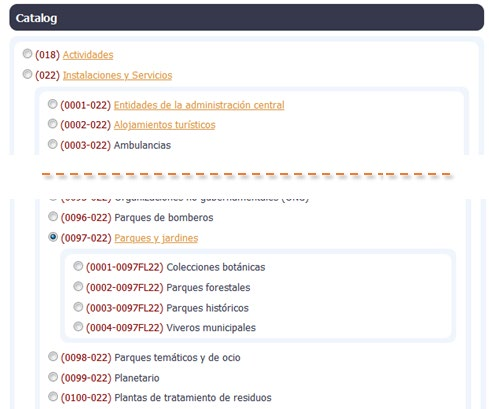
\includegraphics[width=\textwidth]{imagenes/Practica3fig1.jpg}
    \caption{Representación de la estructura jerárquica de los concepts del catálogo de datos.}
    \label{fig:Practica3fig1.jpg}
\end{figure}


La aplicación por desarrollar recibirá como argumento el criterio de búsqueda, esto es, el código de la categoría de la que se desea información, y proporcionará información sobre los concepts y datasets pertinentes, aplicando para ello los siguientes criterios:

\begin{itemize}
    \item Se considerarán pertinentes el concept cuyo código (elemento code) coincida con el criterio de búsqueda y todos los concepts descendientes del mismo.
    \item Se considerarán pertinentes los dataset que contengan información asociada a alguno de los concept pertinentes (contengan un elemento concept con el atributo id igual al atributo id del elemento concept pertinente).
\end{itemize}

La Figura 2 muestra un ejemplo de búsqueda del concept con código 0097-022 y los resultados que se obtendrían.

\begin{figure}[H]
    \centering
    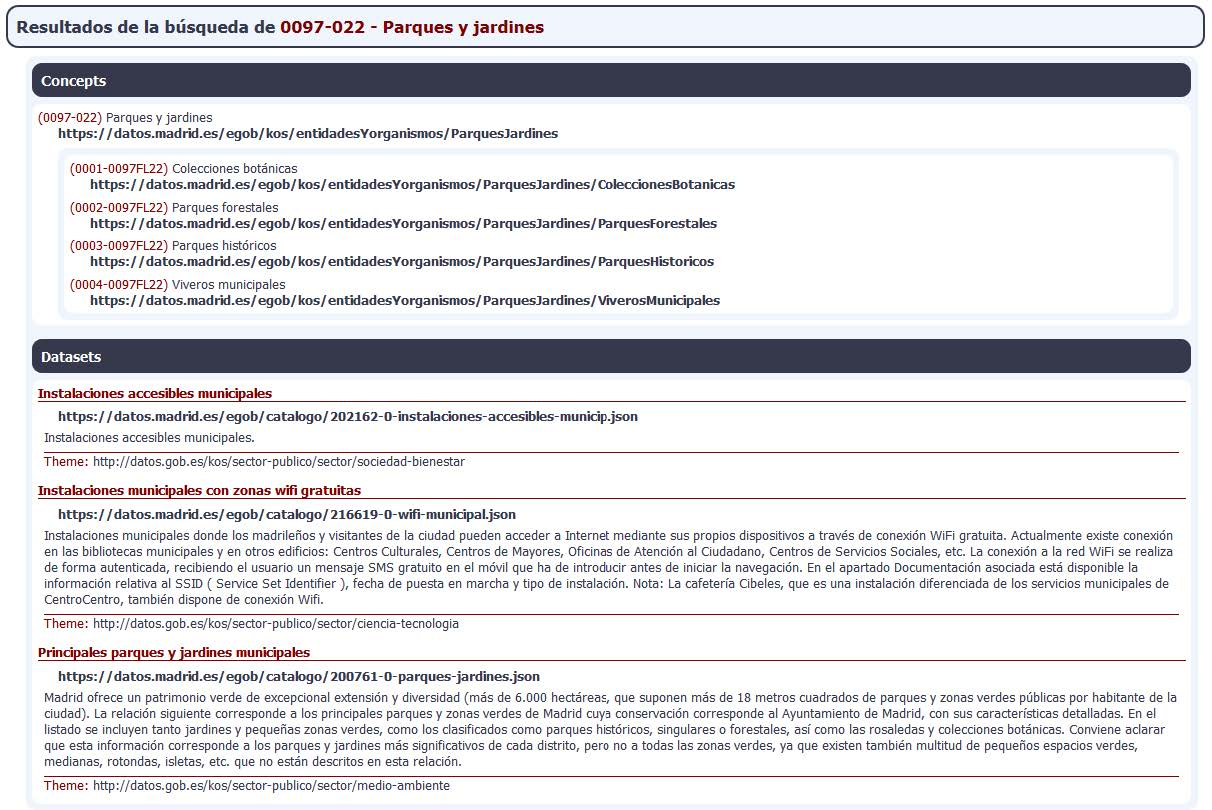
\includegraphics[width=\textwidth]{imagenes/Practica3fig2.jpg}
    \caption{Concepts y datasets pertinentes para el código 0097-022.}
    \label{fig:Practica3fig2.jpg}
\end{figure}

\subsection{Desarrollo de la práctica}

\noindent La implementación de la Práctica 3 se basa en la creación de un analizador de documentos XML denominado XMLParser, desarrollado en JavaCC. Este analizador se ha diseñado para procesar documentos XML que contienen datos publicados en el Portal de Datos Abiertos del Ayuntamiento de Madrid (http://datos.madrid.es).
Los documentos XML que se procesan a través de esta herramienta presentan ciertas características clave, como la identificación de recursos mediante URI, la asociación a categorías, la agrupación en conjuntos de datos y una clasificación jerárquica basada en características temáticas. La tarea principal del analizador es extraer información específica relacionada con códigos de categorías y, posteriormente, generar un nuevo documento XML que contiene los resultados deseados.

El primer paso para resolver la práctica es definir la estructura del analizador que seguirá el procesamiento de los documentos XML. Esta estructura determina cómo se identifican y extraen los datos de los documentos, así como las acciones correspondientes a realizar en cada caso. La siguiente figura ilustra esta estructura:

\textbf{Figura 1: Estructura del analizador XML. Procesamiento de conceptos y datasets.}

Esta figura refleja la estructura del análisis sintáctico, en la que se observa cómo se procesan los elementos concept y dataset. Se observa cómo se manejan los distintos elementos y atributos dentro de cada uno, de tal forma que se describe la estructura de forma detallada. En aquellos no-terminales en los que se quiera ejecutar alguna acción, como puede ser añadir los conceptos y datasets a las listas pertinentes, o crear nuevos objetos de tipo Concept o Dataset, se define una acción léxica dentro del no-terminal, como por ejemplo:

\begin{lstlisting}

Concept concept() : {}
{
  <OPEN_CONCEPT> <ID> idValue = <STRING> <END_ELEMENT>
  <OPEN_CODE> codeValue = getCode() <CLOSE_CODE>
  <OPEN_LABEL> labelValue = getValue() <CLOSE_LABEL>
  (
    <OPEN_CONCEPTS>
    (
      childConcept = concept()
      {
        concepts.add(childConcept);
      }
    )+
    <CLOSE_CONCEPTS>
  )?
  <CLOSE_CONCEPT>
  {
    if(codeValue.equals(nombreCategoria)) {
      conceptLabel = idValue.image;
      conceptsList.add(new Concept(idValue.image, codeValue, labelValue, concepts));
    }
    return new Concept(idValue.image, codeValue, labelValue, concepts);
  }
}

\end{lstlisting}

En este fragmento de código se observa el no-terminal Concept(), el cual define la estructura XML que debe tener un <concept>. Si nos fijamos detenidamente en el procesamiento del no-terminal, podemos apreciar que se realizan dos acciones léxicas: una para añadir a una lista de concepts un concepto hijo (concepts.add(childConcept);), y otra que realiza la comparación del valor de <code> con el nombre de la categoría para crear un objeto concept con los campos extraídos.

\phantom{text}

\noindent \textbf{Estructura del Analizador XMLParser}

\phantom{text}

\noindent El archivo XMLParser.jj define la estructura y funcionamiento del analizador XML mediante JavaCC. A continuación, se describe detalladamente cada componente y su función, proporcionando una comprensión completa del desarrollo y el diseño del analizador.

En las opciones del analizador se definen configuraciones importantes como la concurrencia:

\lstset{inputencoding=utf8/latin1}
\begin{lstlisting}
options
{
  STATIC = false;
}
\end{lstlisting}

Estas opciones configuran el analizador para que no genere métodos estáticos, permitiendo la concurrencia y el procesamiento de múltiples entradas de manera eficiente.

Una vez definidas las opciones del analizador, comienza la declaración del parser y la definición de la clase XMLParser:

\lstset{inputencoding=utf8/latin1}
\begin{lstlisting}
    
PARSER_BEGIN(XMLParser)
package piat.opendatasearch;
import java.util.List;
import java.util.ArrayList;
public class XMLParser {
    private List<Concept> conceptsList;
    private List<Dataset> datasetsList;
    private String conceptLabel;
    private String nombreCategoria;
}
PARSER_END(XMLParser)
    
\end{lstlisting}

en la que se observa que se instacia una lista de objetos Concept, en la que se almacenarán todos los Concept cuyo código coincida con el criterio de la búsqueda, así como los Concept recursivos que puedan tener.
Además se observa otra lista, en este caso de objetos Dataset, en la que igualmente se almacenarán aquellos objetos Dataset que contengan algún un elemento concept con el atributo id igual al atributo id del algún elemento concept de conceptsList.
También se observa la creación de los atributos conceptLabel y nombreCategoría, encargados de almacenar el valor de <label> en cada concept, y de almacenar el valor del nombre de la categoría pasado como argumento al programa principal, respectivamente.

Acto seguido, se definen los tokens que identifican las diferentes etiquetas y elementos del documento XML, así como las reglas para omitir espacios en blanco y caracteres irrelevantes:

\lstset{inputencoding=utf8/latin1}
\begin{lstlisting}
    
SKIP :
{
    " "
| "\t"
| "\r"
| "\n"
}

TOKEN :
{
    < OPEN_CONCEPTS : "<concepts>" >
| < OPEN_DATASETS : "<datasets>" >
| < CATALOG : "<catalog" >
| < XMLNS : "xmlns=" >
| < XMNLNS_XSI : "xmlns:xsi=" >
| < XSI_SCHEMA_LOCATION : "xsi:schemaLocation=" >
| < HEADER : "<?xml version=\"1.0\" encoding=\"UTF-8\"?>" >
| < OPEN_CONCEPT : "<concept" >
| < OPEN_DATASET : "<dataset" >
...
| < VALUE_CODE : ">" (~[ "\"", "\n", "\r", "<", ">", "=" ])+ "<" >
| < VALUE_LABEL : "<![CDATA[" (~[ "\"", "\n", "\r", "<", ">", "=" ])+ "]]>" >
| < STRING : "\"" (~[ "\"", "\n", "\r" ])+ "\"" >
| < END_ELEMENT : ">" >
}

SKIP :
{
    < ~[ ] >
}
    
\end{lstlisting}

Las reglas de omisión aseguran que los espacios en blanco, tabulaciones y saltos de línea no interfieran con el análisis, permitiendo que el analizador se concentre únicamente en los elementos significativos del XML. Se observa también que en caso de que el analizador detecte cualquier cosa que no sea un token que hayamos definido, se omite dicho elemento

\lstset{inputencoding=utf8/latin1}
\begin{lstlisting}

SKIP :
{
    < ~[ ] >

}

\end{lstlisting}

. De esta forma, cualquier token que no hayamos definido se omitirá. Como se estudio en **Estado del arte. javacc.tokens. Se define este token el último ya que este token acepta cualquier carácter, por lo que si no lo ponemos como el último token, se aplicaría la regla 2 y se omitiría todo carácter en el documento, lo que no nos permitiría recoger los token que hemos definido.

\tipbox{En este caso se observa que no se ha empleado ningún estado léxico, esto es debido a que se ha preferido realizar una comprobación estructural del documento ---asi como haría un xsd, aunque de forma mucho mas limitada---. En la practica 5 veremos un analizador XML en el que se sí se hace uso de estados léxicos, y veremos como esta funcionalidad acelera en gran medida el procesamiento.
}

Una vez visto el analisis léxico, toca centrarse en el analizador sintáctico. Este comienza con el método processFile, que recibe como argumento un código de categoría y procesa el archivo XML, extrayendo los conceptos y conjuntos de datos pertinentes:

\lstset{inputencoding=utf8/latin1}
\begin{lstlisting}

ManejadorXML processFile(String code) :
{
    conceptsList = new ArrayList<Concept>();
    datasetsList = new ArrayList<Dataset>();
    nombreCategoria = code;
}
{
    < HEADER > 
    < CATALOG > < XMLNS > < STRING > < XMNLNS_XSI > < STRING > < XSI_SCHEMA_LOCATION > < STRING > < END_ELEMENT >
    (< OPEN_CONCEPTS > (concept())+ < CLOSE_CONCEPTS >)+
    (< OPEN_DATASETS > (dataset())+ < CLOSE_DATASETS >)+
    < CLOSE_CATALOG >
    {
    return new ManejadorXML(datasetsList, conceptsList);
    }
}
    
\end{lstlisting}

Este método inicializa las listas de conceptos y conjuntos de datos, y establece el nombre de la categoría que se utilizará como criterio de búsqueda. Luego, procesa el documento XML siguiendo la estructura definida, identificando y extrayendo los conceptos y conjuntos de datos pertinentes. Al finalizar el procesamiento, retorna un objeto ManejadorXML que contiene las listas de conceptos y conjuntos de datos extraídos.
\tipbox{
    Es importante destacar el sentido que tiene utilizar la clase ManejadorXML, si el parser que estamos desarrollando ya busca lo que quiere. El sentido que tiene es cronológico, ya que primero el parser realiza el análisis del documento y devuelve los datos, si se llama a una función que devuelva los datos es posible que se llamen a estas funciones antes de que se llame a la función de análisis.
}
Como se puede observar en el método, hace referencia a dos no-terminales, los métodos concept() y dataset().
El método concept() procesa cada concepto, extrayendo su código, label y posibles conceptos hijos. Utiliza recursividad para manejar estructuras jerárquicas de conceptos, asegurando que se capturen todas las relaciones parentales y de descendencia.

\lstset{inputencoding=utf8/latin1}
\begin{lstlisting}
    
Concept concept() :
{
  Token idValue;
  String codeValue, labelValue;
  Concept childConcept; 
  List < Concept > concepts = new ArrayList < Concept > ();
}
{
  < OPEN_CONCEPT > < ID > idValue = < STRING > < END_ELEMENT > 
  < OPEN_CODE > codeValue = getCode() < CLOSE_CODE > 
  < OPEN_LABEL > labelValue = getValue() < CLOSE_LABEL >
  (
    < OPEN_CONCEPTS >
    (
      childConcept = concept()
      {
        concepts.add(childConcept);
      }
    )+
    < CLOSE_CONCEPTS >
  )?
  < CLOSE_CONCEPT >
  {
    if(codeValue.equals(nombreCategoria)) {
      conceptLabel = idValue.image;
      conceptsList.add(new Concept(idValue.image, codeValue, labelValue, concepts));
	}
	return new Concept(idValue.image, codeValue, labelValue, concepts);
  }
}

\end{lstlisting}

Concretamente, el método concept se encarga de identificar cada elemento <concept> en el documento XML. Extrae el valor del atributo id, el código del concepto y el label del concepto. Si el código del concepto coincide con el criterio de búsqueda (nombreCategoria), se agrega a la lista de conceptos pertinentes (conceptsList). Además, si el concepto contiene conceptos hijos, el método se llama recursivamente para procesar estos hijos y construir una estructura jerárquica completa.

\textbf{...mencionar explícitamente que la recursividad se utiliza para manejar la estructura jerárquica de los conceptos....}

Por otra parte, si nos centramos en el método dataset(), este  procesa cada conjunto de datos, extrayendo su título, descripción y conceptos asociados. Es responsable de identificar los conjuntos de datos que contienen información relevante para los conceptos identificados previamente.

\lstset{inputencoding=utf8/latin1}
\begin{lstlisting}
    
void dataset() :
{
    Token idDataset, idConcept;
    String title;
    String description = "";
    String keyword = "";
    String theme = "";
    String publisher = "";
    List < IdConcept > idConcepts = new ArrayList < IdConcept > ();
} 
{
    < OPEN_DATASET > < ID > idDataset = < STRING > < END_ELEMENT > 
    < OPEN_TITLE > title = getValue() < CLOSE_TITLE > 
    (< OPEN_DESCRIPTION > description = getValue() < CLOSE_DESCRIPTION >)?
    (< OPEN_KEYWORD >  keyword = getValue() < CLOSE_KEYWORD >)?
    (< OPEN_THEME > theme = getValue() < CLOSE_THEME >)?
    (< OPEN_PUBLISHER > publisher = getValue() < CLOSE_PUBLISHER >)?
    (
    < OPEN_CONCEPTS >
    (
        < OPEN_CONCEPT > < ID > idConcept = < STRING > < END_ELEMENT >
        {
        idConcepts.add(new IdConcept(idConcept.image));
        }
    )+
    < CLOSE_CONCEPTS >
    )?
    < CLOSE_DATASET >
    {
    for(IdConcept ic : idConcepts) {
        if(ic.getId().equals(conceptLabel)) {
        datasetsList.add(new Dataset(idDataset.image, title, description, keyword,theme,publisher,idConcepts));
        }
    }
    }
}   

\end{lstlisting}

Como se puede observar, este no-terminal se encarga de procesar los elementos <dataset> en el documento XML. Extrae el id, el título y otros atributos opcionales como descripción, keyword, theme y publisher. También identifica los conceptos asociados a cada conjunto de datos y los agrega a una lista de identificadores de conceptos (idConcepts). Si alguno de estos identificadores coincide con el conceptLabel pertinente, el conjunto de datos se agrega a la lista de conjuntos de datos pertinentes (datasetsList).

Además, el analizador cuenta con los métodos auxiliares getCode()  y getLabel(). Estos métodos auxiliares extraen el valor de los códigos y labels de los elementos XML. Son utilizados por los métodos concept y dataset para obtener los valores necesarios de los elementos XML.

\lstset{inputencoding=utf8/latin1}
\begin{lstlisting}

String getCode() :
{
    Token t = new Token();
}
{
    (t = < VALUE_CODE >)?
    {
    return t.image.substring(1, t.image.length() - 1);
    }
}

String getValue() :
{
    Token t = new Token();
}
{
    (t = < VALUE_LABEL >)?
    {
    return t.image;
    }
}  

\end{lstlisting}

El método getCode extrae el valor del código de un elemento $<$code$>$ eliminandvo los caracteres $<$ y $>$, mientras que el método getValue extrae el valor de un elemento <label> utilizando la sintaxis CDATA.

\phantom{text}

\noindent \textbf{Funcionalidad del Analizador}

\phantom{text}

% Como se ha visto, XMLParser está diseñado para cumplir con los siguientes requisitos específicos de la práctica:

% Extracción de conceptos relevantes: Identificar y extraer los conceptos cuyo código coincide con el criterio de búsqueda proporcionado, así como todos los conceptos descendientes de estos.
% Identificación de conjuntos de datos pertinentes: Determinar los conjuntos de datos que contienen información relacionada con los conceptos relevantes y extraer esta información.
% Generación de resultados en XML: Crear un nuevo documento XML que incluya los conceptos y conjuntos de datos extraídos, estructurados de manera que faciliten la búsqueda y el análisis posterior.

% El uso de JavaCC para desarrollar este analizador permite una mayor precisión y eficiencia en el procesamiento de documentos XML complejos. JavaCC, al ser una herramienta de generación de compiladores, permite definir de manera precisa las reglas de análisis sintáctico y léxico necesarias para interpretar documentos XML de forma efectiva. Esto es particularmente útil para manejar la complejidad y la jerarquía de los datos XML, asegurando que todos los elementos y relaciones se procesen correctamente.

% Además, la implementación en Java facilita la integración del analizador con otros sistemas y aplicaciones, permitiendo reutilizar el código y extender la funcionalidad según sea necesario. La capacidad de Java para manejar grandes volúmenes de datos y su amplia biblioteca estándar proporcionan una base robusta para el desarrollo de herramientas de análisis de datos.

% En resumen, la implementación de esta práctica proporciona una herramienta poderosa para analizar y extraer información de documentos XML, cumpliendo con los objetivos establecidos y demostrando la efectividad del uso de JavaCC en el desarrollo de analizadores de documentos XML. Esta herramienta no solo cumple con los requisitos de la práctica, sino que también ofrece un ejemplo claro de cómo utilizar técnicas avanzadas de análisis sintáctico y léxico para resolver problemas complejos de procesamiento de datos.

Como se ha visto, XMLParser se ha diseñado para cumplir con los requisitos específicos de la práctica, que incluyen la extracción de conceptos relevantes y la identificación de conjuntos de datos pertinentes.

Una de las funciones principales del analizador es extraer los conceptos que coinciden con el criterio de búsqueda proporcionado, así como todos sus conceptos descendientes. Además, determina los conjuntos de datos que contienen información relacionada con estos conceptos y los extrae para su posterior procesamiento.

Para facilitar la manipulación y el análisis de los datos extraídos, el analizador genera resultados en XML. Esto se realiza creando un nuevo documento XML estructurado de manera que facilite la búsqueda y el análisis posterior de los conceptos y conjuntos de datos.

La implementación del analizador se realiza utilizando JavaCC, lo que permite una mayor precisión y eficiencia en el procesamiento de documentos XML complejos. JavaCC es una herramienta de generación de compiladores que permite definir con precisión las reglas de análisis sintáctico y léxico necesarias para interpretar los documentos XML de manera efectiva. Esta capacidad es crucial para manejar la complejidad y la jerarquía de los datos XML, asegurando un procesamiento correcto de todos los elementos y relaciones.

Además, la implementación en Java facilita la integración del analizador con otros sistemas y aplicaciones. Esto permite reutilizar el código y extender la funcionalidad según sea necesario. La capacidad de Java para manejar grandes volúmenes de datos y su amplia biblioteca estándar proporcionan una base sólida para el desarrollo de herramientas de análisis de datos.

En conclusión, la implementación de esta práctica proporciona una herramienta poderosa para analizar y extraer información de documentos XML. No solo cumple con los objetivos establecidos, sino que también demuestra la efectividad del uso de JavaCC en el desarrollo de analizadores de documentos XML. Esta herramienta ofrece un ejemplo claro de cómo utilizar técnicas avanzadas de análisis sintáctico y léxico para resolver problemas complejos de procesamiento de datos.

% \subsubsection{Preguntas Frecuentes}


% \subsubsection{Notas}

% \tipbox{
% hacer clase concept con atributos code y label, hacer lista concepts de concept. hacer lo mismo con dataset. recoger los datos al igual que hacíamos en NXCalculator
% Concepts, son objetos distintos, se tienen que reconocer de manera diferente. -> Nuevo objeto conceptInDataset
% No hace falta un estado léxico, simplemente crear un objeto nuevo ya que son cosas diferentes, -> IncludedConcepts
% String id -> idConcepts
% XMLParser devuelve un objeto que tenga implementado la interfaz ParserCatalogo
% }

% \noindent Como se ha comentado en la sección anterior, la principal herramienta desarrollada en esta práctica es el analizador XMLParser. Este analizador es capaz de llevar a cabo varias tareas esenciales:

% \begin{itemize}
%     \item Validación de argumentos de entrada para garantizar que los parámetros cumplan con las especificaciones requeridas.
%     \item Extracción de información relevante de los documentos XML, siguiendo las reglas y estructuras definidas en la gramática.
%     \item Generación de documentos de resultados que cumplen con un esquema específico.
% \end{itemize}
% El analizador XMLParser representa una contribución significativa en términos de procesamiento y manipulación de documentos XML.

\subsection{Validación de resultados}

En cuanto a tiempo de ejecución no hay muchas diferencia, el principal aspecto a destacar en esta práctica es la simplicidad con la que se genera el analizador y el potencial de recursividad que este tiene. 
Suponga que se encuentra desarrollando esta práctica utilizando la herramienta SAX. Si la prácticas se modificase ---ligeramente--- y el catalogo.xml tuviese una recursividad mas profunda, esto complicaría mucho el procesamiento Java para algo que a priori no cambia mucho el formato del fichero que se quiere analizar. En otras palabras, un pequeño cambio en el documento a analizar implicaría un gran cambio del programa principal o clase encargada de analizar dicho fichero utilizando SAX.
Sin embargo, empleando JavaCC este problema no existiría. Esto es debido a la recursividad inherente que proporciona la plataforma, permitiendo que dentro de un no-terminal se encuentre especificado ese mismo no-terminal ---lo hemos visto en este capítulo con el método concept(), y lo vimos también en el ejemplo de Calculadora explicado en **estado del arte** con los métodos Expression() y Factor()---. Esto significa que el grado de complejidad del archivo a analizar es inversamente proporcional al grado de complejidad de la gramática a desarollar en JavaCC.

\textbf{...mencionar ejemplos concretos de las ventajas de JavaCC sobre SAX en términos de recursividad y manejo de cambios en la estructura del XML...}

Además, JavaCC permite definir de manera sintáctica el documento objetivo, funcionalidad que SAX no implementa.

\subsection{Conclusiones}

\noindent La Práctica 3 ha brindado a los estudiantes una experiencia valiosa en el manejo de tecnologías de análisis de documentos XML. A través del uso de JavaCC y la tecnología SAX, se ha proporcionado una base sólida para procesar información estructurada de manera eficiente. Los estudiantes han tenido la oportunidad de aplicar conceptos relacionados con la validación de argumentos, el análisis de elementos XML y la generación de documentos de resultados.
Uno de los aspectos más destacados de esta práctica es la capacidad de filtrar y seleccionar información relevante basada en códigos de categorías. Esta habilidad es fundamental en situaciones donde la extracción selectiva de datos es esencial.


\subsection{Código Fuente}

\noindent El código fuente de los archivos elaborados en esta practica se encuentra a continuación para su estudio y aprendizaje. Cabe destacar que se proporcionan dicho código para que el lector sea capaz de probar las funcionalidades con el objetivo de aprender mas acerca de las aplicaciones de JavaCC.

No se promueve el plagio y la realización de las prácticas, este simplemente es una de las muchas formas en las que se podría realizar la práctica.

\hyperref[sec:XMLParser]{XMLParser.jj}
%\href{https://shorturl.at/alqN6}{XMLParser.jj}

\section{Análisis de archivos JSON. Práctica 4}

\noindent La Práctica 4 se centra en la exploración y aplicación de la tecnología GSON Streaming para el análisis y procesamiento eficiente de documentos JSON. El objetivo principal de esta etapa es familiarizar a los estudiantes con la API GSON Streaming y desarrollar un analizador de documentos JSON basado en esta tecnología. Como objetivo secundario, se busca capacitar a los estudiantes en el diseño de algoritmos eficientes para la extracción y transformación de información proveniente de fuentes de contenidos estructurados.

\subsection{GSON Streaming}

\noindent La API de transmisión de GSON es una API de Java que permite leer y escribir JSON de forma secuencial. Esto la hace útil en situaciones donde no es posible o deseable cargar el modelo de objeto completo en memoria, como cuando se trabaja con grandes cantidades de datos o cuando los datos se reciben de forma continua.

La API de transmisión de GSON se basa en dos clases principales: JsonReader y JsonWriter. JsonReader se utiliza para leer JSON de forma secuencial, mientras que JsonWriter se utiliza para escribir JSON de forma secuencial.

Las características principales de la API son su eficiencia en términos de memoria y  su flexibilidad. Por una parte, la API de transmisión de GSON no necesita cargar el modelo de objeto completo en memoria, lo que la hace más eficiente en términos de memoria que la API de GSON tradicional. Además, GSON Streaming permite leer y escribir datos JSON de forma secuencial, lo que la hace muy flexible.

La API es ideal para trabajar con grandes cantidades de datos, ya que puede leer y escribir los datos sin necesidad de cargarlos todos en memoria. También es ideal para recibir datos de forma continua, ya que puede leer los datos a medida que se reciben.


\subsection{JavaCC vs. GSON Streaming}

Mientras que GSON Streaming se basa en un enfoque de lectura secuencial, lo que puede resultar eficiente para grandes volúmenes de datos, JavaCC ofrece la posibilidad de crear analizadores sintácticos personalizados con un control granular sobre el proceso de análisis.

Esta característica resulta fundamental en este contexto, ya que permite la extracción selectiva de la información relevante de los archivos JSON, optimizando el uso de recursos y mejorando el rendimiento general del sistema.

Extracción selectiva: A diferencia de GSON Streaming, que procesa todo el flujo de datos, JavaCC permite definir qué elementos y atributos son relevantes, optimizando el proceso de análisis.
Rendimiento: Al evitar el procesamiento innecesario de información, se reduce el consumo de recursos y se mejora el rendimiento, especialmente al tratar con grandes conjuntos de datos.
Flexibilidad: JavaCC ofrece un alto grado de flexibilidad para adaptarse a diferentes estructuras de archivos JSON, lo que lo convierte en una herramienta versátil para el análisis de datos.

\subsection{Descripción de la práctica}

\noindent La práctica busca ampliar la funcionalidad de la herramienta de búsqueda del Portal de Datos Abiertos del Ayuntamiento de Madrid, desarrollada en la Práctica 3. Se pretende dotar a esta herramienta de la capacidad para extraer información sobre los recursos asociados a una categoría específica (concept) del portal. Esto se logrará accediendo a los conjuntos de datos (dataset) en formato JSON y procesándolos con un analizador GSON Streaming.

% El código desarrollado en la Práctica 3 servirá como punto de partida, y se completará para integrar un analizador GSON Streaming. Este analizador procesará la información de cada conjunto de datos pertinente y generará un documento XML válido conforme al esquema de documento ResultadosBusquedaP4.xsd. El nuevo elemento introducido en este esquema es resources, que contendrá información sobre los recursos asociados a las categorías pertinentes.

% La generación del documento XML (indicado por ARG2) será similar al proceso de la Práctica 3, pero ahora se incorporará el elemento resources. Se utilizará la clase JSONDatasetParser para implementar el analizador GSON Streaming, y se analizarán los archivos .json indicados en el atributo id de cada dataset. Se añadirán como máximo cinco recursos (resource) a partir de cada dataset analizado.


Para ello, se utilizará JavaCC para crear un analizador sintáctico que, a diferencia de GSON Streaming, permitirá la extracción selectiva de los datos necesarios, optimizando el proceso. La información extraída se utilizará para generar un documento XML válido conforme al esquema ResultadosBusquedaP4.xsd, que incluye un nuevo elemento "resources" para almacenar la información sobre los recursos.

\subsection{Desarrollo de la práctica}

La implementación con JavaCC se basa en la definición de una gramática que refleje la estructura de los archivos JSON a analizar. Esta gramática permitirá al analizador identificar los elementos relevantes y extraer la información deseada.

% \subsubsection{Preguntas Frecuentes}

% \noindent Pregunta 1: ¿Cuál es el propósito principal de la Práctica 4 en términos de procesamiento de información JSON?
% Respuesta: El objetivo principal es extender la herramienta de búsqueda para extraer información sobre recursos asociados a categorías específicas en el Portal de Datos Abiertos, utilizando la tecnología GSON Streaming.

% Pregunta 2: ¿Qué elemento se introduce en el esquema Resultados\\BusquedaP4.xsd ?
% Respuesta: Se introduce el elemento resources, que contendrá información sobre los recursos asociados a las categorías pertinentes.

% Pregunta 3: ¿Cuál es la versión de la API GSON Streaming utilizada en esta práctica?
% Respuesta: Se utiliza la versión 2.9.0 de la API GSON Streaming, disponible en este enlace.


\noindent La herramienta principal desarrollada en esta práctica es la extensión de la herramienta de búsqueda del Portal de Datos Abiertos, ahora mejorada con la capacidad de analizar y procesar datos JSON mediante la API GSON Streaming. La clase JSONDatasetParser representa la implementación de este analizador GSON Streaming. La herramienta final permite la extracción selectiva de información de archivos JSON, generando un documento XML conforme al esquema ResultadosBusquedaP4.xsd que incluye el nuevo elemento resources.

\subsection{Validación de resultados}

La validación de los resultados se realizará contrastando la información extraída con la información original de los archivos JSON. Se prestará especial atención a la precisión y completitud de los datos extraídos, así como al rendimiento del analizador implementado con JavaCC.

\begin{figure}[H]
	\centering
	\includegraphics[width=\textwidth]{imagenes/p4jsonvalidacion2.png}
	\caption{\label{fig:p4jsonvalidacion2}Práctica 4. Fichero JSON que analiza JavaCC}
\end{figure}

\begin{figure}[H]
	\centering
	\includegraphics[width=\textwidth]{imagenes/p4xmlvalidacion.png}
	\caption{\label{fig:p4jsonvalidacion2}Práctica 4. Fichero XML que genera el programa}
\end{figure}


\textbf{INSERTAR IMAGEN JSON Y XML}

Se espera que la utilización de JavaCC en lugar de GSON Streaming demuestre las ventajas de esta herramienta en términos de eficiencia, flexibilidad y control sobre el proceso de análisis de datos JSON.

\textbf{INSERTAR IMAGEN FICHEROS FUENTE PARA VER LO SIMPLE QUE ES
}
\textbf{TIEMPOS...}
\textbf{INSERTAR IMAGEN TIEMPOS...EXPLICAR}

\begin{figure}[H]
	\centering
	\includegraphics[width=\textwidth]{imagenes/comparacion_tiempos_ejecucion_p4.png}
	\caption{\label{fig:comparacion_tiempos_ejecucion_p4}Comparación de Tiempos de Ejecución: GSON vs JavaCC}
\end{figure}


\subsection{Conclusiones}

% \noindent La Práctica 4 ha proporcionado a los estudiantes una oportunidad única para aplicar sus conocimientos adquiridos en la Práctica 3 y explorar en profundidad la API GSON Streaming. La capacidad de extender la funcionalidad de la herramienta existente para manejar datos JSON y generar documentos XML enriquecidos demuestra una comprensión avanzada de las tecnologías de procesamiento de datos estructurados.

% El uso de GSON Streaming versión 2.9.0 ha permitido a los estudiantes implementar un analizador eficiente para manejar grandes conjuntos de datos JSON, cumpliendo así con los requisitos de la práctica.

La elección de JavaCC como herramienta principal para el análisis de datos en esta práctica no es casual. En la siguiente práctica ---así como se hizo en la anterior--- se abordará la extracción de información de documentos XML utilizando XPath. La versatilidad de JavaCC permitirá, en la práctica 5, sustituir también esta herramienta, creando un flujo de trabajo unificado y simplificado para el procesamiento de información en diferentes formatos.

\subsection{Código Fuente}

\noindent El código fuente de los archivos elaborados en esta practica se encuentra a continuación para su estudio. Cabe destacar que se proporcionan dicho código para que el lector sea capaz de probar las funcionalidades con el objetivo de aprender mas acerca de las aplicaciones de JavaCC.

No se promueve el plagio y la realización de las prácticas, este simplemente es una de las muchas formas en las que se podría realizar la práctica.

\hyperref[sec:JSONParser]{\textbf{JSONParser.jj}}
%\href{https://shorturl.at/wFG45}{JSONParser.jj}

\section{Análisis de archivos XML (2). Práctica 5}

% La Práctica 5 representa una etapa crucial en el proyecto, enfocándose en la familiarización con la tecnología de transformación de documentos XML mediante el Lenguaje de Rutas de XML (XPath), basado en el Modelo de Objetos de Documento (DOM). El objetivo principal es extraer información del documento XML generado en la Práctica 4 utilizando expresiones XPath y almacenarla en un nuevo documento en formato JSON. Esta práctica permite a los estudiantes explorar técnicas avanzadas de manipulación de datos estructurados.

\noindent La Práctica 5 marca un punto de inflexión en este proyecto, al introducir la transformación de documentos XML mediante XPath (XML Path Language) y el Modelo de Objetos de Documento (DOM). El objetivo principal es extraer información específica del documento XML generado en la Práctica 4 y representarla en formato JSON. Este proceso permite explorar técnicas avanzadas de manipulación de datos estructurados y sienta las bases para la integración con otras herramientas y sistemas.

Sin embargo, en lugar de depender de XPath para la extracción de datos, en este proyecto se propone la utilización de JavaCC como herramienta única para el análisis y procesamiento del documento XML. Esta elección se justifica por la eficiencia, flexibilidad y control que ofrece JavaCC, permitiéndonos prescindir de herramientas adicionales como XPath, SAX o GSON.

\subsection{XPath}

XPath, abreviatura de XML Path Language, es un lenguaje de consulta para documentos XML. Se utiliza para seleccionar partes de un documento XML, como elementos, atributos, texto y datos binarios.

XPath se basa en una sintaxis similar a la de las expresiones regulares. Las expresiones XPath se utilizan para construir caminos a través de un documento XML.

Para ilustrar su uso, consideremos el siguiente fragmento de XML:

\lstset{inputencoding=utf8/latin1}
\begin{lstlisting}
<catalog>
    <concepts>
        <concept
            id="https://datos.madrid.es/egob/kos/...">
            <code>0001-018</code>
            <label><![CDATA[CiudaDistrito]]></label>
        </concept>
    </concepts>
</catalog>

\end{lstlisting}

Si nuestro objetivo fuera seleccionar el código del primer concept, la expresión XPath que utilizaríamos sería:

\lstset{inputencoding=utf8/latin1}
\begin{lstlisting}
/catalog/concepts/concept/code
\end{lstlisting}

Esta expresión realiza un recorrido por el documento desde la raíz (/) hasta el elemento catalog, para luego buscar el elemento concepts, el elemento concept y finalmente seleccionar su hijo code.

Las principales características de XPath son las siguientes:

Selección de elementos: XPath se puede utilizar para seleccionar elementos individuales o conjuntos de elementos en un documento XML.
Selección de atributos: XPath se puede utilizar para seleccionar atributos individuales o conjuntos de atributos de un elemento.
Selección de texto: XPath se puede utilizar para seleccionar texto de un elemento o atributo.
Selección de datos binarios: XPath se puede utilizar para seleccionar datos binarios de un elemento o atributo.

XPath se utiliza en una variedad de aplicaciones, incluyendo el procesamiento de XML, el desarrollo web, y la integración de datos. Esto permite que se utilize para procesar documentos XML, extraer datos, validar documentos y transformar documentos. Además, se utiliza en aplicaciones web para acceder a datos XML, como datos de formularios o datos de un servicio web. Por último, también se puede emplear para integrar datos de diferentes fuentes, como datos XML y datos de bases de datos.

\subsection{JavaCC vs. XPath}

\noindent Tanto JavaCC como XPath pueden emplearse para procesar documentos XML, sin embargo, cada uno presenta características que los hacen más adecuados para diferentes escenarios.

JavaCC es una herramienta de generación de analizadores sintácticos. Se utiliza para generar analizadores sintácticos que pueden analizar documentos XML.

Como ya hemos visto en secciones anteriores, las principales ventajas de JavaCC son su eficiencia en términos de memoria y su gran flexibilidad a los usuarios. Por otra parte, la principal desventaja de JavaCC es su dificultad de uso,

XPath es un lenguaje de consulta para documentos XML. Se utiliza para seleccionar partes de un documento XML.

Las principales ventajas de XPath son su sencillez, ya que es una herramienta relativamente sencilla de aprender a utilizar, y su generalidad, pues se puede utilizar para procesar cualquier documento XML, independientemente de su lenguaje.

Las principales desventajas de XPath son su eficiencia, debido a que es menos eficiente en términos de memoria que JavaCC, y sus limitaciones, como la imposibilidad de procesar datos binarios.


\subsection{Descripción de la práctica}

\noindent Esta práctica se basa en la extensión del código desarrollado en la Práctica 4, sustituyendo la utilización de XPath por un nuevo analizador desarrollado en JavaCC. El objetivo principal es procesar un nuevo fichero XML, extrayendo información específica que se almacenará en un documento JSON.

Para lograr este objetivo, se implementará un nuevo analizador léxico y sintáctico en JavaCC que nos permita:

Identificar los elementos relevantes: El analizador debe ser capaz de reconocer las etiquetas y atributos específicos del documento XML que contienen la información a extraer.
Extraer la información: Una vez identificados los elementos relevantes, el analizador debe extraer su contenido y almacenarlo en estructuras de datos apropiadas.
Generar el documento JSON: Finalmente, el analizador debe utilizar la información extraída para generar un nuevo documento en formato JSON con la estructura deseada.

% \noindent La implementación de la Práctica 5 se basa en extender el código desarrollado en la Práctica 4, integrando la funcionalidad de XPath para extraer información específica del documento XML resultante. El uso del Modelo de Objetos de Documento (DOM) facilita la navegación y manipulación de la estructura jerárquica del documento XML.

% Se requerirá la introducción de expresiones XPath para identificar y seleccionar los elementos deseados en el documento XML. La información obtenida mediante XPath se almacenará en un nuevo documento en formato JSON. Este proceso de transformación garantiza que la información relevante se extraiga eficientemente y se represente en un formato JSON para su posterior análisis o intercambio.

% En esta práctica, se llevará a cabo la evaluación de las sentencias XPath sobre el documento XML de salida generado en la práctica anterior. Este documento será utilizado para realizar varias consultas específicas que permitirán extraer datos relevantes. Las consultas XPath incluirán la obtención del contenido textual del elemento <query>, el conteo de elementos <dataset> hijos de <datasets>, la extracción del contenido de cada elemento <title> hijo de <resource>, y la identificación del número de elementos <resource> cuyo atributo id coincide con el atributo id del elemento <dataset>.

% A la hora de implementar esta funcionalidad utilizando XPATH, en el guión de la práctica se recomienda desarrollar una nueva clase  responsable de evaluar las expresiones XPath y devolver una colección con los resultados. La estos resultados serán convertido a formato JSON. Finalmente, el documento JSON generado contendrá todos los resultados de las evaluaciones XPath en el formato especificado.

% Además, en el guión se menciona que el proyecto continuará utilizando las clases implementadas en prácticas anteriores ---en nuestro caso, implementaremos los mismos parsers XML y JSON que vimos en las secciones de las prácticas 3 y 4 respectivamente---, y se integrará una nueva clase principal renombrada como P5\_XPATH, que incluirá el código necesario para cumplir con las nuevas especificaciones. La aplicación deberá recibir argumentos adicionales que incluyan la ruta al documento JSON de salida.

% Este ejercicio refuerza la familiarización con XPath y DOM, destacando la importancia de las tecnologías de transformación y manipulación de documentos XML en aplicaciones telemáticas. Además, la práctica provee una comprensión práctica de cómo estas tecnologías pueden ser utilizadas para realizar consultas avanzadas y transformar datos XML en formatos más manejables y adecuados para el análisis o intercambio de información.

\subsection{Desarrollo de la práctica}

\noindent La herramienta principal desarrollada en esta práctica es una extensión del código existente en la Práctica 4, sustituyendo la capacidad de utilizar expresiones XPath para extraer información específica del documento XML con un nuevo parser desarrollado en JavaCC para analizar un nuevo fichero XML. La información extraída se guarda en un nuevo documento en formato JSON, ofreciendo una representación alternativa y flexible de los datos.

En esta sección, vamos a describir cómo se resuelve esta práctica utilizando JavaCC y XPath, apoyándonos en el archivo XMLParser2.jj proporcionado.

\phantom{text}

\noindent \textbf{Configuración del Analizador}

\phantom{text}

Se mantienen las opciones del analizador utilizadas en las prácticas anteriores, garantizando la compatibilidad y la posibilidad de analizar las tres gramáticas (P3, P4, P5) con el mismo parser.

\lstset{inputencoding=utf8/latin1}
\begin{lstlisting}
options
{
    STATIC = false; // para permitir entradas de manera dinámica
    JAVA_TEMPLATE_TYPE = "modern"; // uso de plantilla moderna de Java
}
\end{lstlisting}


Además, también hay que declarar del parser y la definir la clase XMLParser2:
\lstset{inputencoding=utf8/latin1}
\begin{lstlisting}
PARSER_BEGIN(XMLParser2)
package piat.opendatasearch;
import java.util.List;
import java.util.ArrayList;
import java.util.HashMap;
public class XMLParser2 {
  private HashMap<String, Integer> datasetsMap;
  private int numDatasets;
  private List<String> titleList;
}
PARSER_END(XMLParser2)
\end{lstlisting}

Esta clase contiene un mapa para almacenar los datasets (datasetsMap), una variable para contar el número de datasets (numDatasets), y una lista para almacenar los títulos (titleList). La estructura de esta clase es fundamental para organizar y gestionar los datos extraídos de los documentos XML de manera eficiente.

La parte mas relevante de este ejercicio con JavaCC es la definición de los tokens y los estados léxicos. Estos permiten acotar el reconocimiento de tokens a secciones específicas del documento, optimizando el proceso de análisis.


\lstset{inputencoding=utf8/latin1}
\begin{lstlisting}
< DEFAULT, QUERY2>
SKIP :
{
  " " 
| "\t"
| "\r"
| "\n"
} 

< DEFAULT >
TOKEN :
{
  < OPEN_DATASETS : "<datasets>" > : IN_DATASETS
| < OPEN_RESOURCES : "<resources>" > : IN_RESOURCES
| < HEADER : "<?xml version=\"1.0\" encoding=\"UTF-8\"?>" > : IN_HEADER
| < OPEN_QUERY : "<query>" > : IN_QUERY
| < CLOSE_SEARCH_RESULTS : "</searchResults>" >
| < CLOSE_CONCEPT : "</concept>" >
}

<IN_HEADER>
TOKEN:
{
 < SEARCH_RESULTS : "<searchResults" >
| < XMLNS : "xmlns=" > 
| < XMNLNS_XSI : "xmlns:xsi=" > 
| < XSI_SCHEMA_LOCATION : "xsi:schemaLocation=" > 
| < END_ELEMENT : ">" > : DEFAULT
}

<IN_QUERY>
TOKEN :
{
 < CLOSE_QUERY : "</query>" > : DEFAULT
}

<IN_DATASETS>
TOKEN : 
{
  < CLOSE_DATASETS : "</datasets>" > : DEFAULT
| < OPEN_DATASET : "<dataset" > : IN_DATASET
}

<IN_RESOURCES>
TOKEN:
{
  < CLOSE_RESOURCES : "</resources>" > : DEFAULT
| < OPEN_RESOURCE : "<resource id=" > : IN_RESOURCE
}

<IN_RESOURCE>
TOKEN:
{
  < CLOSE_RESOURCE : "</resource>" > : IN_RESOURCES
| < OPEN_CONCEPT : "<concept id=" > 
| < OPEN_TITLE : "<title>" >  : IN_TITLE
}

<IN_TITLE>
TOKEN:
{
 < CLOSE_TITLE : "</title>" > : IN_RESOURCE
}

< IN_DATASET >
TOKEN:
{
 < CLOSE_DATASET : "</dataset>" > : IN_DATASETS
| < ID : "id=" >
}

< IN_HEADER, IN_DATASET, IN_RESOURCE>
TOKEN:
{
< STRING : "\"" (~[ "\"", "\n", "\r" ])+ "\"" >
}

<IN_TITLE, IN_QUERY>
TOKEN:
{
  < VALUE : (~["<"])+ > 
}

<*>
SKIP :
{
  < ~[ ] >
}
\end{lstlisting}

Como en las prácticas anteriores, omitimos los espacios en blanco, tabulaciones y saltos de linea. En este caso, incorporamos estados léxicos, que nos permiten reconocer un grupo de tokens en un punto específico del análisis. 
El uso principal de los estados léxicos en la práctica es para reconocer unicamente lo que nos interesa del documento, que es la cabecera del documento, el valor del documento <query>, el valor id de cada dataset, y el valor title de cada resource. 
Los estados léxicos definidos, además del estado DEFAULT son:

\begin{itemize}
    \item IN\_HEADER: estado utilizado para reconocer únicamente elementos de la cabecera del archivo, como el espacio de nombres, la version XML, o la localización del XMLSchema. Se crea este estado principalmente para poder reconocer los strings dentro de la cabecera como se hacía en la práctica 3.
    \item IN\_QUERY: estado utilizado para reconocer el contenido del elemento query.
    \item IN\_TITLE: estado utilizado para reconocer el contenido del elemento title.
    \item IN\_DATASETS: estado utilizado para reconocer los elementos id dentro de la estructura de un dataset
    \item IN\_RESOURCES: Estado utilizado para reconocer el id de los recursos y el valor del elemento title dentro de la estructura de un resource
\end{itemize}

\textbf{...explicar con más detalle la lógica detrás de la elección de cada estado y su función específica en el análisis del XML...DIAGRAMA-TABLA...}

\tipbox{
    Cabe destacar que se definen los estados lexicos mencionados para omitir el resto de caracteres o token que el analizador pueda reconocer en un momento dado. Por ejemplo, después de la cabera solo nos interesa el elemento query, por lo que definimos un estado lexico IN\_QUERY en el que definimos los tokens que nos permiten reconocer el valor de la query. De esta forma, se definen ciertos tokens que unicamente pueden o deben ser analizados en un punto concreto del analisis.
}

Una vez se definen los tokens, resta generar el análisis sintáctico. El método principal processfile() inicializa las estructuras de datos y procesa el archivo XML, extrayendo la información relevante y almacenándola en las estructuras adecuadas:

\lstset{inputencoding=utf8/latin1}
\begin{lstlisting}
void processFile() : { String s; datasetsMap = new HashMap<>(); titleList = new ArrayList<String>(); }
{
  < HEADER > 
  < SEARCH_RESULTS > < XMLNS > < STRING > < XMNLNS_XSI > < STRING > < XSI_SCHEMA_LOCATION > < STRING > < END_ELEMENT > 
  < OPEN_QUERY > s = getCode() < CLOSE_QUERY > { System.out.println(s); }
  < OPEN_DATASETS > (dataset())* < CLOSE_DATASETS >
  < OPEN_RESOURCES > (resource())* < CLOSE_RESOURCES >
  {
    System.out.println("[NUM_DATASETS] " + numDatasets);
    System.out.println("[MAP]: " + datasetsMap);
    System.out.println("TITLE: " + titleList);
  }
}

\end{lstlisting}

Este procesa el documento XML siguiendo la estructura definida, identificando y extrayendo los datos pertinentes. Al finalizar el procesamiento, imprime el número de datasets, el mapa de datasets, y la lista de títulos extraídos.

Además, se cuenta con el método dataset() que procesa cada dataset, extrayendo su id y actualizando el mapa de datasets:

\lstset{inputencoding=utf8/latin1}
\begin{lstlisting}

void dataset() : { Token idDataset; } 
{
  < OPEN_DATASET > < ID > idDataset = < STRING > 
  < CLOSE_DATASET >
  {
    datasetsMap.put(idDataset.image.replace("\"", ""), 0);
    numDatasets++;
  }
}
\end{lstlisting}

El método dataset identifica cada elemento <dataset> en el documento XML, extrae su id y lo agrega al mapa de datasets, incrementando el contador de datasets.

Además, también se cuenta con el método resource(), que procesa cada recurso, extrayendo su id, el id del concepto asociado, y el título. También actualiza el contador de conceptos en el mapa de datasets:

\lstset{inputencoding=utf8/latin1}
\begin{lstlisting}
void resource() : { Token idResource, idConcept; String title; } 
{
  < OPEN_RESOURCE >  idResource = < STRING > 
  < OPEN_CONCEPT >  idConcept = < STRING>
  < OPEN_TITLE > title = getCode() < CLOSE_TITLE > 
  < CLOSE_RESOURCE >
  {
    titleList.add(title);
    if (datasetsMap.containsKey(idResource.image.replace("\"", ""))) {
        // If key exists, increments corresponding value
        int contador = datasetsMap.get(idResource.image.replace("\"", ""));
        datasetsMap.put(idResource.image.replace("\"", ""), contador + 1);
    } 
  }
}
\end{lstlisting}


% \subsubsection{Preguntas Frecuentes}

% \noindent Pregunta 1: ¿Cuál es el propósito principal de la Práctica 5 en términos de transformación de datos?
% Respuesta: El objetivo principal es la extracción de información específica del documento XML mediante expresiones XPath y la posterior representación de esta información en un nuevo documento en formato JSON.

% Pregunta 2: ¿Cómo se realiza la transformación de datos de XML a JSON en esta práctica?
% Respuesta: La transformación se realiza mediante la utilización de expresiones XPath para identificar y seleccionar información específica en el documento XML generado en la Práctica 4. La información seleccionada se almacena en un nuevo documento en formato JSON.

% Pregunta 3: ¿Cómo se integra la funcionalidad XPath en el código existente de la Práctica 4?
% Respuesta: Se realizarán modificaciones en el código de la Práctica 4 para incorporar expresiones XPath que seleccionen la información deseada. La información extraída se utilizará para generar un nuevo documento en formato JSON.

\subsection{Validación de resultados}

Para validar los resultados de la Práctica 5, se llevan a cabo diversas comprobaciones. Se realiza una comparación visual del JSON generado para verificar que la información extraída del XML se haya almacenado correctamente, con la estructura y los valores esperados. Se presta especial atención a la correspondencia entre los elementos del XML y las claves del JSON, así como a la integridad de los datos.

\textbf{INSERTAR IMAGEN XML Y JSON}

Se valida el formato JSON utilizando un validador online o una herramienta de desarrollo para asegurar que el JSON generado cumple con la sintaxis correcta y no contiene errores.

\textbf{INSERTAR IMAGEN VALIDADOR ONLINE. añadir texto explicativo}

\begin{figure}[H]
	\centering
	\includegraphics[width=\textwidth]{imagenes/p5validacionjsonrfc.png}
	\caption{\label{fig:p5validacionjsonrfc}Práctica 5. Comprobación del archivo JSON generado en la herramienta online \textit{JSON Formatter \& Validator} }
\end{figure}

Para garantizar la robustez de la solución, se prueba la aplicación con diferentes archivos XML de entrada, con diferentes estructuras y contenidos, asegurando así que la extracción de información mediante XPath funciona correctamente en diferentes escenarios.

Finalmente, se analiza el tiempo de ejecución de la aplicación con archivos XML de diferentes tamaños para comprobar que la extracción de información mediante XPath se realiza de forma eficiente. En aspecto no se observa una diferencia notable entre las dos herramientas.

\begin{figure}[H]
	\centering
	\includegraphics[width=\textwidth]{imagenes/p5tiemposejecucion.png}
	\caption{\label{fig:p5tiemposejecucion}Comparación de Tiempos de Ejecución: XPath vs JavaCC}
\end{figure}

\textbf{INSERTAR GRÁFICO TIEMPOS JAVACC Y XPATH. COMPLETAR CON TEXTO
}

\subsection{Conclusiones}

\noindent La Práctica 5 demuestra el potencial de JavaCC como herramienta única para el análisis y procesamiento de documentos XML en el contexto de las aplicaciones telemáticas. La capacidad de integrar el análisis léxico, el análisis sintáctico, la extracción de información y la generación de documentos en un único framework simplifica el desarrollo y ofrece un mayor control sobre el proceso. 

% \noindent La Práctica 5 proporciona a los estudiantes una valiosa experiencia en la utilización de JavaCC para la extracción selectiva de información de documentos XML. La capacidad de integrar esta tecnología con el código existente de la Práctica 4 demuestra la versatilidad en el manejo de datos estructurados.

% El proceso de transformación a JSON destaca la flexibilidad de la tecnología utilizada, permitiendo la representación de datos en diferentes formatos según las necesidades del proyecto.

La sustitución de XPath por JavaCC en esta práctica no solo simplifica la arquitectura de la solución, sino que también abre la puerta a la implementación de funcionalidades más complejas y personalizadas en el futuro.

\section{Evolutivo de las prácticas}

\subsection{Introducción}

\noindent Como se ha podido observar de las prácticas de las secciones anteriores, pese a ser interesantes y cumplir con los objetivos establecidos de aprendizaje, son poco interesantes y se podría realizar unos ejercicios mas potentes y versátiles que exprimiesen al máximo las funcionalidades de las herramientas que hemos ido repasando.

Es por ello que en esta sección se plantea unos ejercicios a modo de evolutivo, que amplían los requerimientos y complejidad del análisis. Además se observará que, gracias al incremento en la complejidad de los ejercicios, aumenta en proporción la sencillez con la que se resuelven dichos problemas empleando JavaCC.

De esta forma, se podrá observar lo ventajoso de crear un analizador a la medida de usuario, y como JavaCC es una herramienta versátil y muy potente.

\tipbox{
    plantear un problema mas interesante y hacer un archivo mas complejo
-las practicas son aburridas, proponer practicas mas interesantes, potentes, versátiles…para demostrar lo fácil que es con javacc, para que se vea la ventaja

}

\subsection{Evolutivo 1. XML}

\noindent Este evolutivo se presenta a partir de la Practica 3. En dicha práctica se analizaban documentos xml, y se proponía analizar un documento xml con cierta recursividad